\section{Bad Pixel Determination}
\label{chap:algorithms:bpm}

\subsection{Detailed Description of the various Algorithms}

%TO BE WRITTEN (SDPG)
%\subsubsection{Bad-pixel detection on a single image}
%TO BE WRITTEN (SDPG)
%\subsubsection{Bad-pixel detection on a stack of images}
%TO BE WRITTEN (SDPG)
%\subsubsection{Bad-pixel detection on a sequence of images}
%TO BE WRITTEN (SDPG)
%
%
%\subsubsection{Cosmic Ray Hits detection}
%
%TO BE WRITTEN (SDPG)
%
%
%\subsection{Performance}
%TO BE WRITTEN (SDPG)

\subsubsection{Bad-pixel detection on a single image}

The {\tt hdrl\_bpm\_2d} recipe identifies bad pixels on individual
images by comparing the value in each pixel with those of the
neighbouring pixels, via two methods.

In method 1 the algorithm first smooths the single image by applying
a cpl-filter (default: median), then subtracts the smoothed images and
derives the bad pixels by scaling the rms with specified thresholds on
the residual image.

Method 2 is similar to method 1, but the smoothed image is obtained
via a Legendre polynomial fit to the image.  More details are given in
Section \ref{sec:bpm_2d}.


We tested the 2 methods on flat fields exposures on sky (both
simulated with artificial bad pixels and real exposures). We found the
following:

\begin{itemize}
\item {\bf Method 1.}  The best performances (missed detections = 0\%,
  false positives = 0\%, recovered bad pixels = 100\%), are obtained
  by setting the recipe parameters to use large smoothing windows
  (i.e. {\tt --bpm.smooth\_ x/y = 49}), relatively high sigma clipping
  levels ({\tt --bpm.kappa\_low/high > 5}), and dilation
  post-filtering with {\tt --pfx/y = 3}. On the contrary, the number of
  false detection increases dramatically. Figure~\ref{fig:single_m1}
  shows the results on simulated flat fields.

\item {\bf Method 2.}  The best performances ($>95$\% success rate)
  are obtained with the sigma clipping levels {\tt
    --bpm.kappa\_low/high = 3}, although this generates a false
  detection rate of 10\%. The number of false detections can be
  lowered by increasing {\tt --bpm.kappa\_low/high}, but but the
  success rate decreases and the number of missed detection increases
  consequentially. The order of the fitting polynomial surface has no
  strong impact on the performances. Figure~\ref{fig:single_m2} shows
  the results on simulated flat fields.

\end{itemize}


\begin{figure} 
 \subfigure
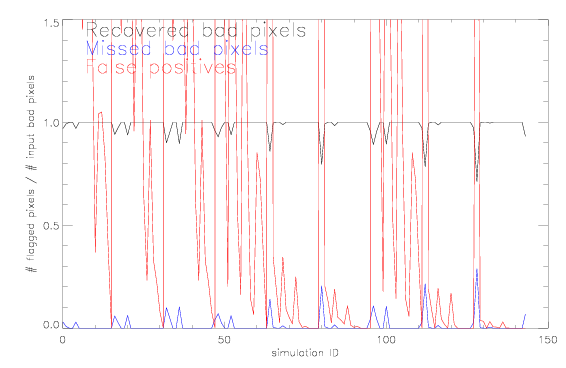
\includegraphics[width=17cm]{figures/recovered_bad_pixels_m1.png}
 \caption{Fraction of recovered bad pixels (black), missed bad pixels
   (blue) and false detections (red) on simulated flat fields using
   method 1 of the {\tt hdrl\_bpm\_2d} recipe. The best performances
   are obtained setting {\tt --bpm.smooth\_x/y =49}, {\tt
     --bpm.kappa\_low/high > 5}, and {\tt --pfx/y =3}. A large
   fraction of false detection is found for {\tt --bpm.smooth\_ x/y
     <5} (corresponding to the run ID that have peaks in the red curve
   in the above figure).}
\label{fig:single_m1}
\end{figure}


\begin{figure}
 \subfigure
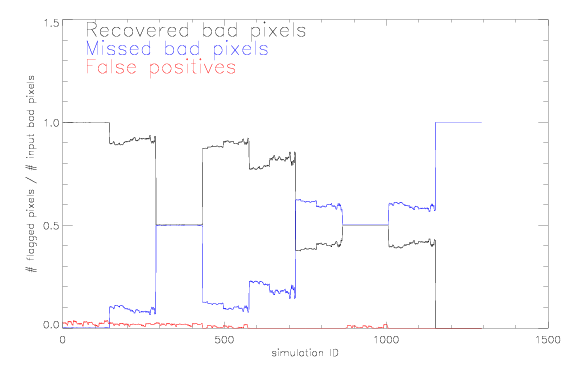
\includegraphics[width=17cm]{figures/recovered_bad_pixels_m2.png}
 \caption{Fraction of recovered bad pixels (black), missed bad pixels
   (blue) and false detections (red) on simulated flat fields using
   method 2 of the {\tt hdrl\_bpm\_2d} recipe. The best performances
   are obtained setting {\tt --bpm.kappa\_low/high = 3} (run ID $<
   100$). For larger values, the number of detected bad pixels
   decreases.}
\label{fig:single_m2}
\end{figure}



\subsubsection{Bad-pixel detection on a stack of images}

The {\tt hdrl\_bpm\_3d} recipe identifies bad pixels on a stack of
images. It compares the value in each pixel of the image $i$-th, with
the same pixel in the other $N-1$ images. It returns a $N$ bad pixel
map cube, with the 3rd axis of dimension $N$.

It has 3 methods, which are detailed in Section ? In a nutshell: 

Method 1 identifies bad pixels using an absolute threshold on
the residual images. The threshold depend strongly on the input data,
and needs to be fine tuned case by case in order to select the best
parameters.

Method 2 identifies bad pixels using a threshold on scaled rms. Method
3 identifies bad pixels by scaling the propagated error of each
individual pixel and compares it with the measured residuals.

Method 2 and 3 have been tested on simulated bias and simulated flat
fields. Both methods have a success rate $> 99$\% in identifying the
bad pixels. Method 3 tends to miss 50\% of the bad pixels if
{\tt --bpm.kappa $\geq$ 10} (method 2 does not have this problem on
the same images), whereas method 2 has a $\sim 6$\% false detection
rate on noise images (method 3 does not have this problem on the same
images).

Figures \ref{fig:stack_m2} and \ref{fig:stack_m3} show the tests on
methods 2 and 3 on noiseless simualted stack of flat fields.


\begin{figure}
 \subfigure
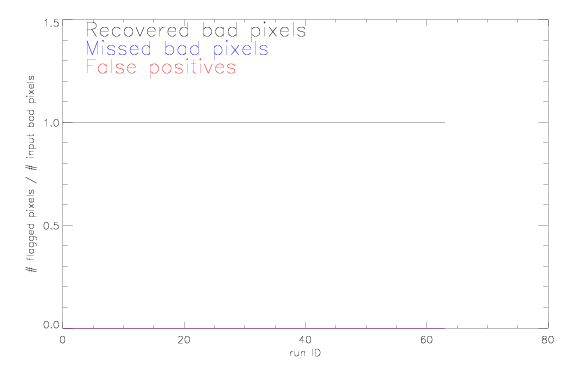
\includegraphics[width=17cm]{figures/recovered_bad_pixels_3d_m2.png}
 \caption{Fraction of recovered bad pixels (black), missed bad pixels
   (blue) and false detections (red) on simulated flat fields, using method 2 of the {\tt hdrl\_bpm\_3d} recipe.}.
 \label{fig:stack_m2}
\end{figure}


\begin{figure}
 \subfigure
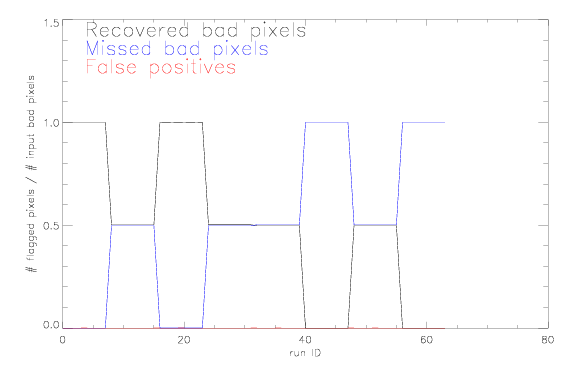
\includegraphics[width=17cm]{figures/recovered_bad_pixels_3d_m3.png}
 \caption{Fraction of recovered bad pixels (black), missed bad pixels
   (blue) and false detections (red) on simulated flat fields, using
   method 3 of the {\tt hdrl\_bpm\_3d} recipe. 50\% of input bad pixels are missed
   if {\tt --bpm.kappa\_low/high > 10}.}
\label{fig:stack_m3}
\end{figure}



\subsubsection{Bad-pixel detection on a sequence of images}

The {\tt hdrl\_bpm\_fit} recipe is targeted to the analysis of a set
of $N$ frames with different exposure time (e.g.  dome flats). At each
position $(x, y)$, bad pixels in each frame are identified via a
polynomial fit of all the $N$ pixels at position $(x, y)$. The header
keyword {\tt EXPTIME} is used as to sampling position of the $N$
pixels along the fit.


{\it Warning}: the routine does not disentangle between i) bad pixels
or non-linear pixel (i.e. ``persistent'' bad values of the same pixel
across the stack of images) and ii) ``accidental'' bad pixel values
(i.e.  the pixel itself is good, but in one frame it has a deviant
value because, for example, of a cosmic ray event). If a pixel in the
sequence of images is flagged in one frame (e.g. a cosmic ray hit it)
but it is not on the other frames, it is flagged in the final mask.

It is therefore advisable to remove cosmic rays on individual frames,
before running {\tt hdrl\_bpm\_fit} on a sequence of images.


The  {\tt hdrl\_bpm\_fit}  recipe has 4 methods:

\begin{itemize}
\item {\bf Method 1.} ({\tt --abs-rchi2-low/-high}): This method marks pixels
  as bad by using the absolute reduced chi squared (low/high)
  threshold: pixels with values below/above this threshold are marked
  as bad. This method needs to be fine-tuned for each dataset, because
  it refers to absolute chi2 values.
                                                                             
\item {\bf Method 2.} ({\tt --rel-rchi2-low/-high}): This method marks
  pixels as bad by using the relative reduced-chi-squared (low/high)
  threshold: pixels with values below/above this threshold times
  measured-rms are marked as bad.
                                                                             
\item {\bf Method 3.} ({\tt --rel-coef-low/-high}): This method marks pixels
  as bad by using the relative coefficient (low/high) threshold:
  pixels with values below/above this threshold times measured-rms are
  marked as bad.
                                                                             
\item {\bf Method 4.}  ( {\tt --pval}): This method uses the p-value
  (between 0\% and 100\%) to discriminate between good and bad pixels.
  Fits with a p-value below the threshold are considered to be bad
  pixels.

\end{itemize}

Figures~\ref{fig:sequence_m2}, \ref{fig:sequence_m3}, and
\ref{fig:sequence_m4} show the results of tests performed on a
sequence of simulated flat fields. Method 2 and 3 tend to miss a large
fraction of bad pixels for {\tt --rel-rchi2} and {\tt --rel-coef}
larger than 1 (which correspond to the first run ID in the mentioned
figures).  Method 4 gives the best performances, independently of the
input {\tt --pval} value.

\begin{figure}
 \subfigure
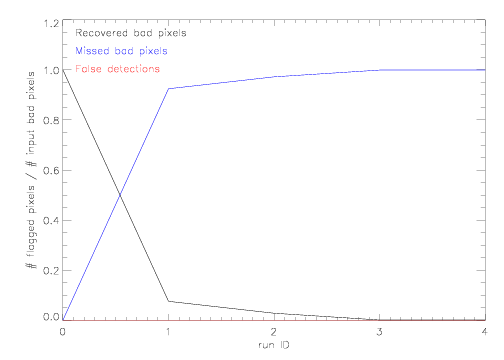
\includegraphics[width=15cm]{figures/results_2.png}
 \caption{Fraction of recovered bad pixels (black), missed bad pixels
   (blue) and false detections (red) on simulated flat fields, using
   method 2 (--rel-rchi2) of the {\tt hdrl\_bpm\_fit} recipe. The best
   performance (run ID=0) corresponds to {\tt --rel-rchi2 = 1}.}
 \label{fig:sequence_m2}
\end{figure}


\begin{figure}
 \subfigure
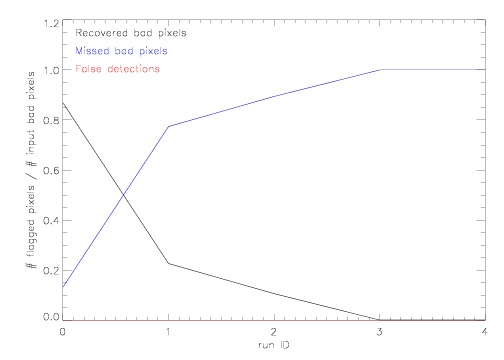
\includegraphics[width=15cm]{figures/results_3.png}
 \caption{Fraction of recovered bad pixels (black), missed bad pixels
   (blue) and false detections (red) on simulated flat fields, using
   method 3 (--rel-coef) of the  {\tt hdrl\_bpm\_fit}  recipe. The best
   performance (run ID=0) corresponds to {\tt --rel-coef = 1}.}
 \label{fig:sequence_m3}
\end{figure}


\begin{figure}
 \subfigure
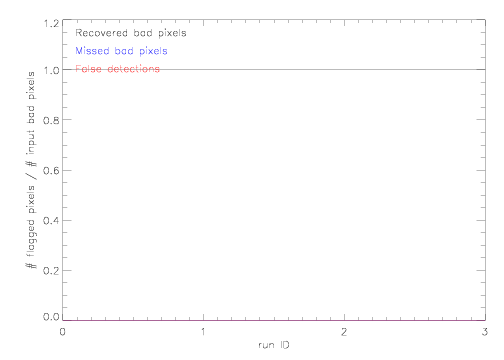
\includegraphics[width=15cm]{figures/results_4.png}
 \caption{Fraction of recovered bad pixels (black), missed bad pixels
   (blue) and false detections (red) on simulated flat fields, using
   method 4 ({\tt --pval}) of the {\tt hdrl\_bpm\_fit} recipe.}
 \label{fig:sequence_m4}
\end{figure}


Driven by robustness of method 4, we tested it on a series of real
flat fields obtained with FORS2 and CRIRES. The test is aimed to
confirm that the number of detected bad pixels is nearly independent
of the adopted {\tt --pval} in {\tt hdrl\_bpm\_fit}. Figure~\ref{fig:sequence_m4_real} indicates indeed
that this is the case: the number of detected bad pixels does not vary
significantly in the range 0.001 < {\tt --pval} < 0.1. Therefore, the defaul
value {\tt --pval = 0.001} can be adopted for most applications.

\begin{figure}
 \subfigure
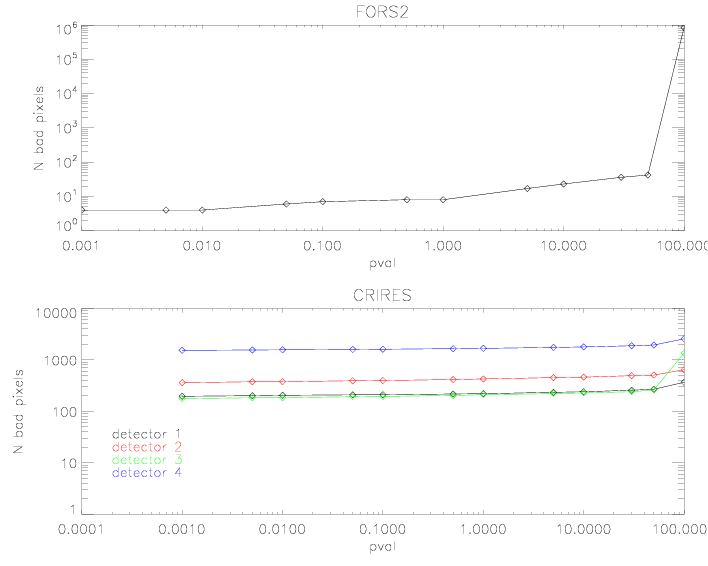
\includegraphics[width=15cm]{figures/results_bpmfit_real.png}
 \caption{Number of flagged bad pixels with {\tt hdrl\_bpm\_fit},
   method 4 as a function of the {\tt --pval} on a series of internal
   flats for FORS2 (upper panel) and CRIRES (lowe panel). The number
   of detected bad pixels does not vary significantly within {\tt
     0.001 < --pval < 0.1}.}
 \label{fig:sequence_m4_real}
\end{figure}


\subsubsection{Cosmic Ray Detection}


The cosmic ray detection algorithm is derived from the LACosmic routine (\cite{vanDokkum2001}).
LACosmic is based on a variation of Laplacian edge detection which uses the sharpness of the
edges of cosmic rays to discriminate between legitimate sources and cosmic rays.   A detailed
description of the algorithm, the default parameters, and applicable data cases
are summarized in \cite{vanDokkum2001}.

In summary, the {\em hdrldemo\_bpm\_lacosmic} routine has the following input parameters:\\

\begin{tabbing}

\quad\= --lacosmic.sigma\_lim\quad  \= structure image that a point must have to be flagged as a cosmic ray. 
\quad \= Default Value Used\kill\\
\> {\bf Parameter}			\>  {\bf Description}					\> {\bf Default Values}       \\
\>  --ext-r                	\>  FITS extension of the RAW. 				\>0      \\
\>  --ext-e               	\>  FITS extension of the ERROR. 				\>0      \\
\>  --ext-b               	\>   FITS extension or the input BPM. 				\>0      \\
\>  --gain                	\>  Gain in [e- / ADU]. 						\>2.5      \\
\>  --ron                 	\>  Read-Out Noise. 							\>1.0      \\
\>  --pfx                 	\>  X Size of the post filtering kernel. 					\>3      \\
\>  --pfy                 	\>   Y Size of the post filtering kernel. 				\>3      \\
\>  --pfm                 	\>   Post filtering mode. [closing or dilation] 				\> closing      \\
\>  --region-llx          	\>   Lower left x pos. (FITS) defining the region. 				\>1      \\
\>  --region-lly          	\>   Lower left y pos. (FITS) defining the region. 				\>1      \\
\>  --region-urx          	\>   Upper right x pos. (FITS) defining the region. 				\>0      \\
\>  --region-ury          	\>  Upper right y pos. (FITS) defining the region. 				\>0      \\
\>  --lacosmic.sigma\_lim  	\>   Poisson fluctuation threshold to flag cosmic rays. 				\>4.5      \\
\>  --lacosmic.f\_lim     	\>   Minimum contrast between the Laplacian image and the fine   \> \\
\>                                   \> structure image that a point must have to be flagged as a cosmic ray.                 \>  2.0 \\
\>  --lacosmic.max\_iter   	\>   Max number of iterations. 				\>5      \\

\end{tabbing}


The User can expect to achieve detection efficiencies of about 90\% on well-sampled images.   This is discussed
in detail in section \ref{sect:testing_CR}.

A good strategy is to run the routine on a typical image using the default parameter values, and then to load the
input image and the resultant cosmic ray detection mask into a display and blink the images.  By slightly varying
the parameters {\em lacosmic.sigma\_lim} and {\em lacosmic.f\_lim} the User can balance the optimal detection
efficiency versus spurious cosmic ray detections.

The detection efficiency and the number of spurious cosmic ray detections can be expected to worsen in data that
is under-sampled.   This may also be true for long slit spectra in which the source spectrum is very sharp.



\subsubsection{Testing the Cosmic Ray Detection}
\label{sect:testing_CR}

The defining parameters of any cosmic ray detection algorithm is its detection efficiency 
(the ratio of the number of cosmic rays found by the routine divided by the total number of cosmic rays), 
the number of spurious detections, and how the total number of cosmic rays and the background environment 
affects the detection.  Therefore, all testing was done by creating a known 
number of cosmic rays of various intensity, size, and shape, and adding these to three different synthetic 
images: an empty field with a Poisson noise distribution, a sparse star and galaxy field, and a dense globular 
cluster field.  The number of cosmic rays was allowed to vary from 50, affecting 300 pixels and covering 0.007\% of 
the field, up to 10,000 cosmic rays, affecting 61,000 pixels and covering 1.5\% of the image.
The recipe was then run on 3 $\times$ 37 = 111 images, stepping between these two extremes of cosmic ray density, and the input cosmic ray 
frames were compared to the detections achieved with the {\em hdrldemo bpm lacosmic} routine. The cosmic ray detection rate was 
a good 89.4\% $\pm$ 0.4\% for the empty and sparse fields, all the way out to unrealistic cosmic ray covering factors of 1.5\%. 
In general, the detection efficiency in the very dense images was, on average, only about 0.3\% worse at a level of 89.1\% $\pm$ 0.4\%. 
The fraction of spurious cosmic ray detections are at a level of about 6.8\% $\pm$ 0.3\% over the full range of cosmic ray densities.

As is evident in figure~\ref{fig:detect_efficiency}, the cosmic ray detection rate is at a level of 
89.4\% $\pm$ 0.4\% for the empty and sparse fields, all the way out to the extremely high cosmic ray covering factors of 1.5\%.   
There is no significant difference in the detection efficiency for the empty images and the sparse fields.
For the very dense images the detection efficiency is not notably worse and is, on average, at a level of 89.1\% $\pm$ 0.4\%.    
The difference between the dense fields and the sparse and empty fields is roughly constant at about 0.3\%.   	
 
Beyond a cosmic ray covering factor of 0.1\%, however, the detection efficiency remains remarkably constant all the way to the 
most densely populated cosmic ray fields.  In this range of covering factors, the number of affected cosmic ray pixels goes 
from 4,000 to 61,000.


\begin{figure}[t]
 \subfigure
\centering
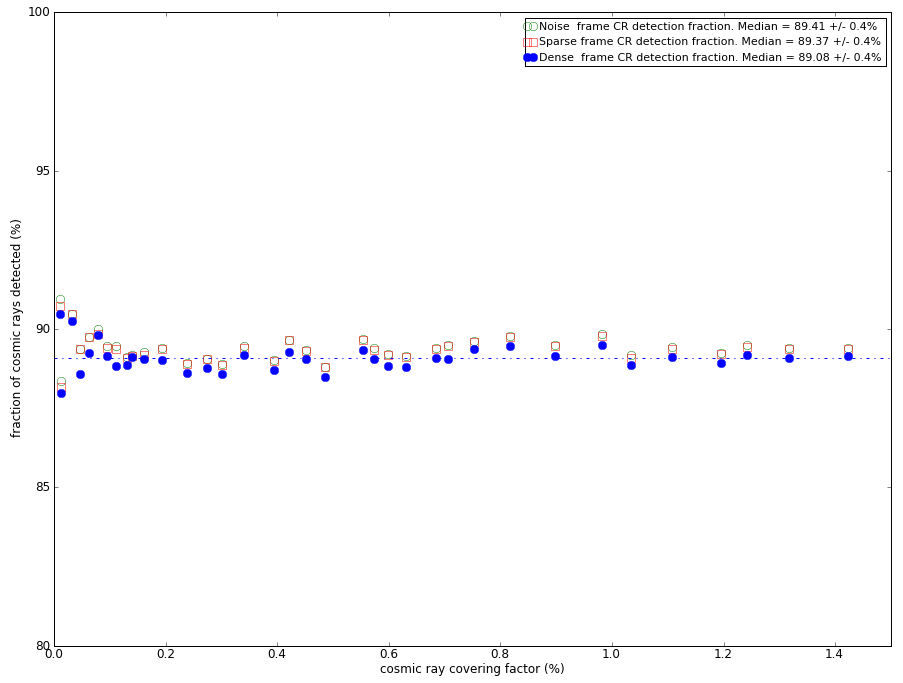
\includegraphics[width=12cm]{figures/LACosmic_det_eff.png} 
%\vspace*{-0.5cm}
\caption[]
	{\footnotesize  The detection efficiency of {\em hdrldemo bpm lacosmic} versus the cosmic ray covering factor (in percent).  The efficiency (given in percent) is measured
	from the number of cosmic rays detected by {\em hdrldemo bpm lacosmic} when applied to the pure noise frame (open green circles), the sparsely populated frame (red squares),
	and the dense frame (solid blue circles).  The average detection rates for the pure background and sparse frames are very similar at 89.4\% $\pm$ 0.4\%, while
	the detection rates in the dense globular cluster frame is always slightly lower at an average of 89.1\% $\pm$ 0.4\%.  The detection efficiency remains remarkably
	constant from cosmic ray covering factors of about 0.1\% to 1.4\% (i.e. from 4,000 to 61,000 affected pixels).
	}
	\label{fig:detect_efficiency}
\end{figure}



The inverse of figure~\ref{fig:detect_efficiency} is given by the fraction of input cosmic rays not detected (see figure~\ref{fig:not_detected}). 
The total count of undetected cosmic rays (figure~\ref{fig:not_detected}, bottom plot) is made independently of the number of detections and is,
therefore, included. Again, for the full range of cosmic ray covering factors, the non-detection rate is about 10.6\% $\pm$ 0.4 for the empty and sparse fields, 
and 11.0\% $\pm$ 0.4\% for the very dense field.

\begin{figure}[b]
 \subfigure
\centering
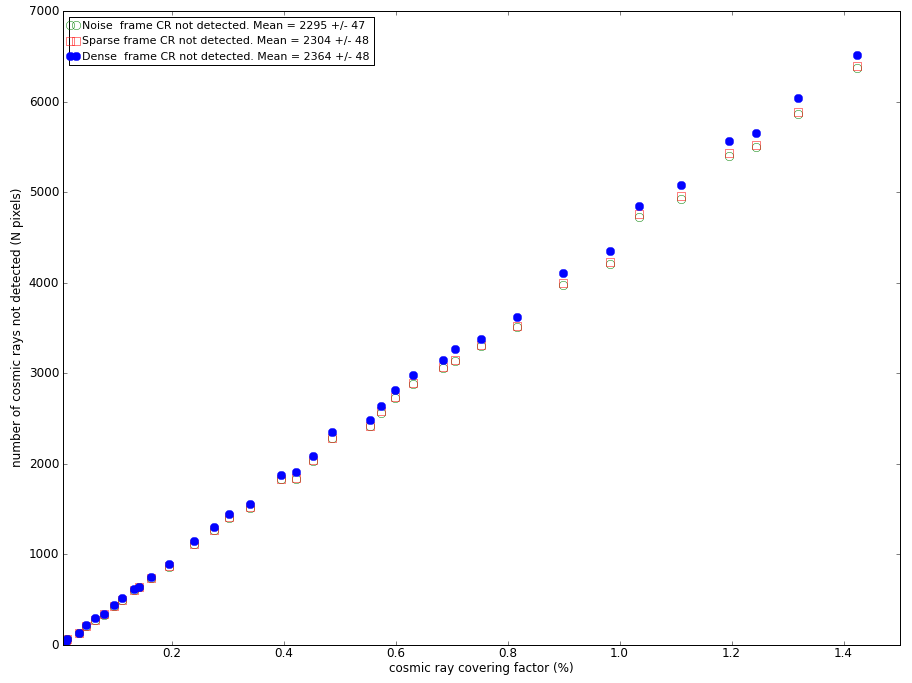
\includegraphics[width=12cm]{figures/LACosmic_not_detA.png} 
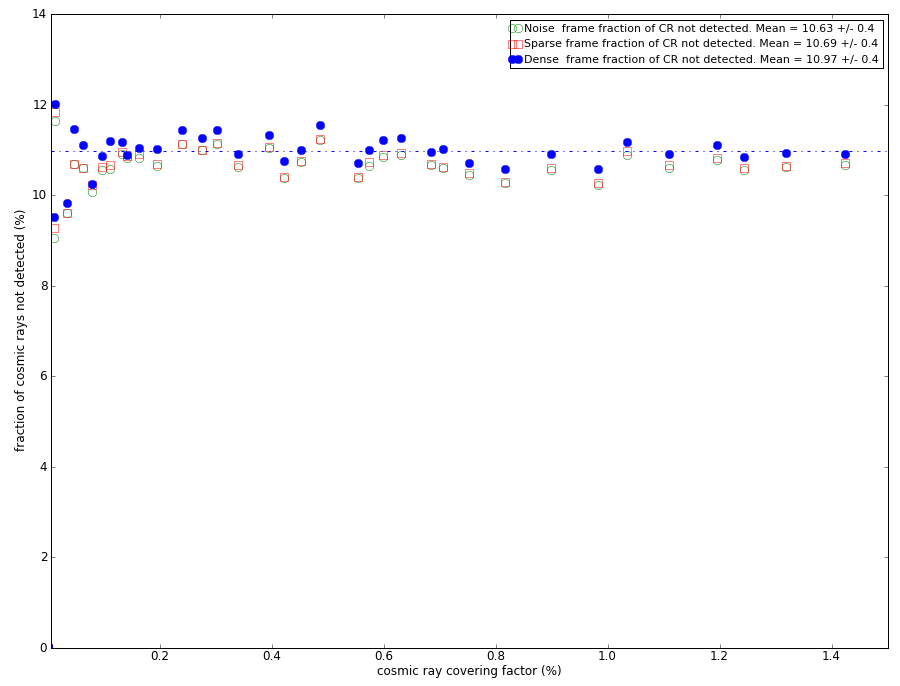
\includegraphics[width=12cm]{figures/LACosmic_not_detB.png}
\caption[]
	{\footnotesize  The number of cosmic rays {\bf not} detected (top panel) and the non-detection fraction (bottom panel) versus the cosmic ray covering factor
	(given in percent).
	}
	\label{fig:not_detected}
\end{figure}


Finally, a count of cosmic rays was made that were detected by {\em hdrldemo bpm lacosmic}, but that do not exist in the original input image (see figure~\ref{fig:spurious}).
The fraction of spurious cosmic ray detections are large for very low covering factors, but this is simply due to the small total numbers
of cosmic rays.   Beyond a covering factor of about 0.2\%, the fraction of spurious cosmic ray detections settles down to a value of about 6.8\% $\pm$ 0.3\%.
Within this regime, the numbers of false-positive detections are virtually indistinguishable between the empty, the sparse, and the dense
fields.

\vspace*{-0.5cm}
\begin{figure}[b]
 \subfigure
\centering
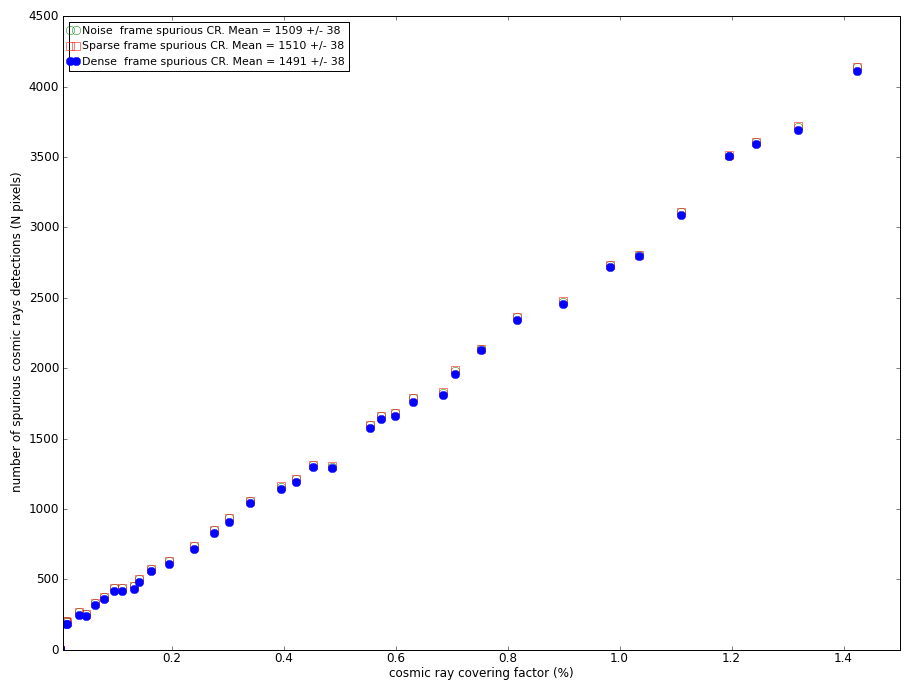
\includegraphics[width=13.3cm]{figures/LACosmic_spuriousA.png} 
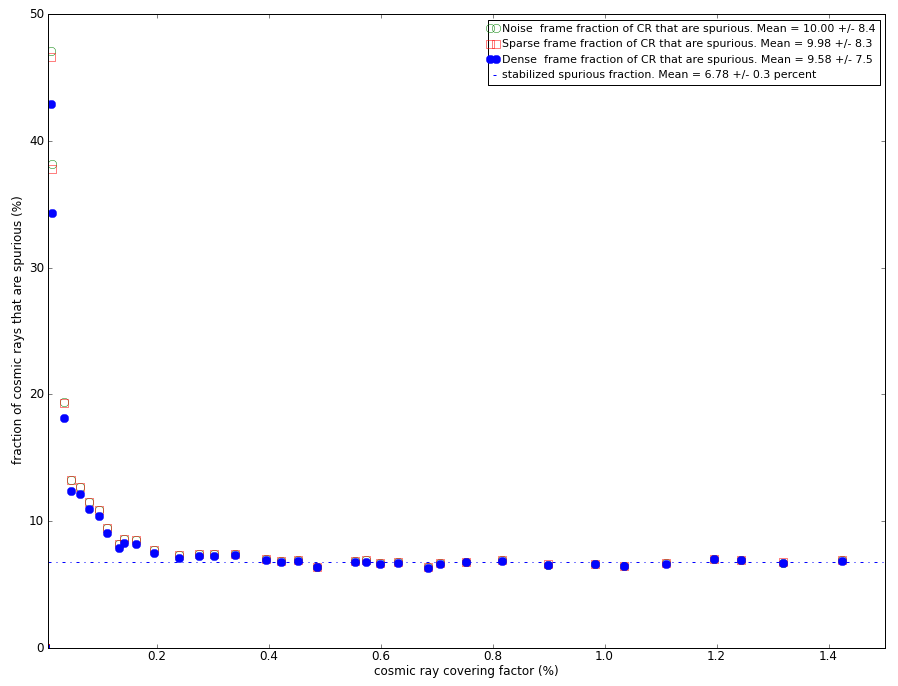
\includegraphics[width=13.3cm]{figures/LACosmic_spuriousB.png}
\caption[]
	{\footnotesize  The number of spurious cosmic ray detections (top panel) and the spurious fraction (bottom panel) versus the cosmic ray covering factor
	(given in percent).
	}
	\label{fig:spurious}
\end{figure}



